\chapter{Kako je kvasac postao proizvo\dj ač vina}
\setbookcodestyle

\section{Uvod}

Jedan od prvih organizama koje su ljudi pripitomili jeste kvasac. Naučnici su 2011. godine u jednoj pećini u Jermeniji otkrili 6000 godina staru vinariju, sa sve presama za gro\v z\dj e, posudama za fermentaciju, pa čak i čašama za piće. Ova vinarija je bila velika tehnološka inovacija za koju je bilo potrebno znati kako kontrolisati \textit{Saccharomyces}, rod kvasca koji se koristi u proizvodnji alkohola i hleba. Me\dj utim, naše interesovanje za alkohol je možda i starije. Naučnici su 2008. godine otkrili da su tupaje, koje su slične drevnim precima svih primata, alkoholičari.  One vole da piju tzv. palmino vino koje se pravi od cveća Bertram palmi. Fermentaciju obavlja kvasac \textit{Saccharomyces} koji živi u tim cvetovima. Ovo otkriće sugeriše da naše interesovanje za alkohol datira milionima godina unazad.

Količina palminog vina koju tupaje konzumiraju bila bi smrtonosna za većinu sisara. Na sreću, one su razvile efikasne načine za metabolizovanje alkohola, i, samim tim, izbegavanje opijanja, što bi povećalo rizik da ih ubije predator.
Zbog tolerancije na alkohol, naučnici veruju da tupaje imaju neke evolutivne prednosti, kao što je zaštita od srčanog udara.

Tako\dj e je veoma moguće da su neki skoriji preci primata bili ljubitelji alkohola. Poznato je da šimpanze piju prirodno fermentisan voćni nektar, kao i da smo od predaka nasledili povezanost izme\dj u unosa alkohola i gojenja. 

\section{Koji geni kvasca su odgovorni za pravljenje vina?}
\subsection{Kako je kvasac postao proizvo\dj ač vina?}

Vrsta kvasca koja će biti razmatrana u ovom poglavlju je  \emph{Saccharomyces cerevisiae}, koja može da pravi vino tako što pretvara glukozu iz voća u alkohol (Slika \ref{slika 1}). Počećemo sa jednostavnim pitanjem: Zašto proizvo\dj ači vina drže grož\dj e u zapečaćenim buradima?
\begin{figure}[h]
    \centering
    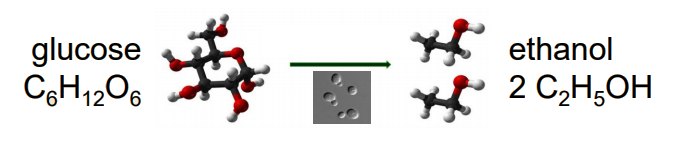
\includegraphics[width=\textwidth]{bio1.png}
    \caption{glukoza $\rightarrow$ etanol}
    \label{slika 1}
\end{figure}

Kada zalihe glukoze nestanu, kvasac mora nešto da uradi da bi preživeo. Kvasac invertuje svoj metabolizam i  etanol postaje njegova nova hrana. Ova inverzija, zvana \textbf{diauxic smena}, može jedino da se desi u prisustvu kiseonika. Ako proizvodjači vina ne zapečate svoja bureta, kvasac u buretu bi svario etanol koji je upravo proizveden, uništavajući vino.

Diauxic smena je složen proces koji dosta utiče na izražavanje mnogih gena. Sledeće pitanje na koje je potrebno dati odgovor je: Koji geni su odgovorni za diauxic smenu?

\subsection{Koji geni su odogovorni za diauxic smenu}
Zamislite vreme kad su prve biljke sa voćem evoluirale, ali nije bilo organizama koji bi metabolizovali datu glukozu iz voća i iskoristili prednost od proizvdenog etanola. Ti organizmi bi imali veliku evolucionu prednost, ali metabolizovanje glukoze, bez obzira na etanol, nije jednostavan zadatak. Diauxic smena zahteva stvaranje potpuno novih metaboličkih puteva koji uključuju mnogo gena koji rade zajedno.

Jedan od mnogih procesa koji kvasac obavlja pri ferementaciji je konverzija iz etanala u etanol. Ako je nekim slučajem prisutan i kiseonik može doći i do obrnute konverzije iz etanola u etanal. Za bilo koju od ovih konverzija odgovoran je enzim Alkohol dehidrogenaza (Adh), za čiju aktivnost su u kvascu odgovorna dva gena koja potiču od istog roditeljskog gena. 

Postmatranjem $n$ gena kvasca kroz $m$ trenutaka sa bilo koje strane diauxic smene, dobijamo $n \times m$ \textbf{matricu ekspresije} gena $E$, gde je $E_{i,j}$ broj koji predstavlja nivo ekspresije gena $i$ u trenutnku $j$. $i$-ti red se zove \textbf{vektor ekspresije} gena $i$. Samo posmatranjem ovih vektora možemo uočiti različite šablone ponašanja gena u zavisnosti od diauxic smene.

\subsection{Uvod u klasterovanje}
Godine 1997. Joseph DeRisi je konstruisao prvu veliku matricu ekspresije gena kvasca \textit{Saccharomyces cerevisiae} uzorkovanjem 7 puta kroz trenutke -6, -4, -2, 0, +2, +4 i +6, gde trenutak 0 pokazuje diauxic smenu. Kako u pomenutom kvascu postoji negde oko 6400 gena, eksperiment rezultira matricom veličine 6400 x 7 (Slika \ref{slika 2}). 
\begin{figure}[h]
    \centering
    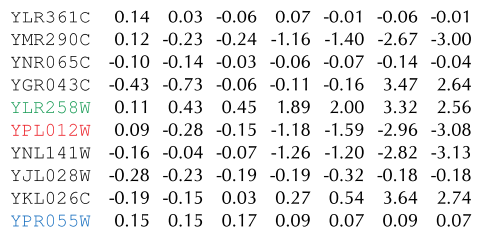
\includegraphics[width=10cm]{bio3.png}
    \caption{Deo matrice ekspresije gena kvasca}
    \label{slika 2}
\end{figure}

Primetimo da ekspresioni vektor gena YPR055W ostaje ravan tokom diauxic smene, na osnovu toga zaključujemo da on ne učestvuje u smeni. Sa druge strane primećujemo da se ekspresioni vektor YLR258W značajno menja tokom diauxic smene, na osnovu toga zaključujemo da je on uključen u smenu. U praksi se obično uzimaju logaritamske vrednosti (Slika \ref{slika 3}). Nakon te transformacije, pozitivne vrednosti u vektoru odgovaraju povećanoj ekspresiji, a negativne smanjenoj ekspresiji.
\begin{figure}[h]
    \centering
    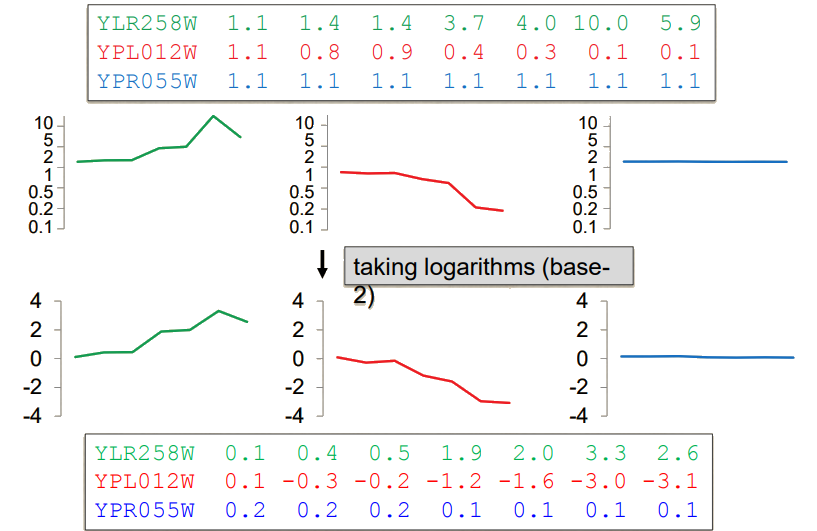
\includegraphics[width=\textwidth]{bio2.png}
    \caption{Ekspresioni vektori 3 gena}
    \label{slika 3}
\end{figure}

\subsubsection{Klasterovanje gena kvasca}
Cilj je da podelimo skup svih gena kvasca u $k$ razdvojenih klastera, tako da geni u istom klasteru imaju slične ekspresione vektore. U praksi broj klastera nije unapred poznat, zbog toga biolozi primenjuju algoritme klasterovanja za različite vrednosti $k$. Zbog jednostavnosti pretpostavićemo da je vrednost $k$ fiskirana. Na slici \ref{slika 4} je prikazana podela gena na tri klastera koji ukazuju na rastuću (zelenu), opadajuću (crvenu) i ravnu (plavu) ekspresiju tokom diauxic smene.
\begin{figure}[h]
    \centering
    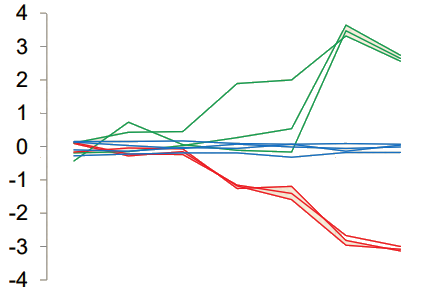
\includegraphics[width=8cm]{bio4.png}
    \caption{Podela gena na 3 klastera}
    \label{slika 4}
\end{figure}

Nivo ekspresije mnogih gena kvasca se neznatno menja pre i posle diauxic smene (plave linije na slici \ref{slika 4}). Tako\dj e, ovi geni imaju osobinu da su sve vrednosti njihovih vektora ekspresije veoma blizu $0$. U našoj analizi isključujemo sve gene kod kojih su vrednosti izme\dj u $-2.3$ i $2.3$. Ovim smanjujemo broj razmatranih gena sa 6400 na 230. Naš zadatak je da klasterujemo ove gene na osnovu sličnog ponašanja.


\section{Klasterovanje kao optmizacioni problem}
\subsection{Dobar princip klasterovanja}
Da bismo identifikovali grupe gena sa sličnim uzorcima(vektorima) ekspresije, zamislimo ekspresioni vektor dužine $m$ kao tačku u $m$-dimenzionom prostoru. Geni sa sličnim vektorima ekspresije 
formiraće klaster. Klasteri bi trebalo da zadovoljavaju sledeći princip.

\textbf{Dobar princip klasterovanja}: Elementi istog klastera bliži su jedni drugima nego što su elementi različitih klastera (slika \ref{slika 5}).

\begin{tcolorbox}
\textbf{Problem dobrog klasterovanja:} Podela skupa tačaka u klastere.\\
\textit{Ulaz:} Skup od n tačaka u m-dimenzionom prostoru i ceo broj k.\\
\textit{Izlaz:} Podela n tačaka u k klastera koji zadovoljavaju princip dobrog klasterovanja.
\end{tcolorbox}

\noindent Napomena: Bilo koja podela na dva klastera ne zadovoljava ovaj princip.
\begin{figure}[h]
    \centering
    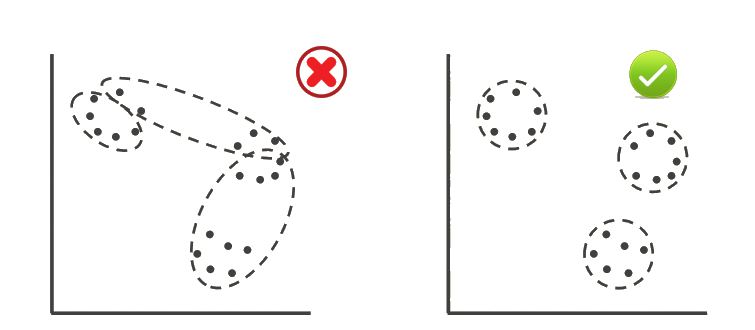
\includegraphics[width=12cm]{bio5.png}
    \caption{Dobar princip klasterovanja}
    \label{slika 5}
\end{figure}

\subsection{Klasterovanje kao optimizacioni problem}

Umesto što mislimo o klasterovanju kao o podeli tačaka podataka $Data$ u $k$ klastera, probajmo da odredimo skup $Centers$ od $k$ tačaka koje predstavljaju \textbf{centre} klastera. Za centre uzimamo one koje minimizuju neku funkciju rastojanja izme\dj u skupova $Centers$ i $Data$ me\dj u svim mogućim centrima (slika \ref{slika 6}). Kako ćemo definisati tu funkciju rastojanja?

Neka su dati tačka $DataPoint$ iz višedimenzionog prostora i skup od k tačaka $Centers$. Rastojanje od tačke $DataPoint$ do $Center$ definišemo kao euklidsko rastojanje od $DataPoint$ do najbližeg centra.

$$d(DataPoint, Centers) = \min_{\text{all points }x\text{ from Centers}} d(DataPoint, x)$$ 
\begin{figure}[h]
    \centering
    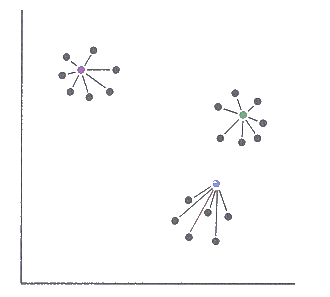
\includegraphics[width=7cm]{bio9.png}
    \caption{Skup tačaka $Data$ sa slike 5 (crne tačke) zajedno sa 3 centra koji formiraju skup $Centers$ (obojene tačke)}
    \label{slika 6}
\end{figure}

Definišimo sada rastojanje izme\dj u svih tačaka podataka $Data$ i centara $Centers$. Označavamo ga sa $MaxDistance(Data, Centers)$ i predstavlja maksimum rastojanja $d(DataPoint, Centers)$ me\dj u svim tačkama $DataPoint$.
$$MaxDistance(Data, Centers) = \max_{\text{all points }DataPoint\text{ from }Data} d(DataPoint, Centers)$$

Sada možemo preformulisati naš problem.

\begin{tcolorbox}
\textbf{Problem k-centar klasterovanja:} Od datog skupa tačaka podataka, naći k centara tako da se minimizuje $MaxDistance(Data, Centers)$.\\
\textit{Ulaz:} Skup tačaka $Data$ i ceo broj $k$.\\
\textit{Izlaz:} Skup $Centers$ od $k$ centara koji minimizuju $MaxDistance(DataPoints, Centers)$ uzimajući u obzir sve moguće izbore centara.
\end{tcolorbox}

\subsection{Farthest Fast Traversal}
Problem kod ovako definisanog problema je to što je NP-težak. Zato ćemo u nastavku opisati heuristiku Farthest Fast Traversal koja bira centre iz skupa tačaka $Data$.
Kao prvi centar bira se proizvoljna tačka iz skupa $Data$. Zatim se iterativno dodaje novi centar kao tačka iz $Data$ koja je najudaljenija od do sada izabranih centara.

Pogledajmo primer na slici \ref{slika 7}. U gornjem levom delu slike smo uzeli proizvoljnu tačku i izabrali je za centar (plava tačka). Za sada sve tačke pripadaju jednom klasteru. U gornjem desnom uglu slike crveno je označen novi centar, tj. najudaljenija tačka od plave tačke. Sada imamo dva klastera. Do novog centra (zelena tačka) smo došli tako što smo računali najmanje rastojanje izme\dj u svake tačke i prva dva centra i primetili da zelena tačka ima najveće rastojanje. Ovo je prikazano u donjem levom uglu slike. Iterativno dolazimo i do četvrtog centra (ljubičasta tačka), koji je prikazan u donjem desnom delu.
\begin{figure}[h]
    \centering
    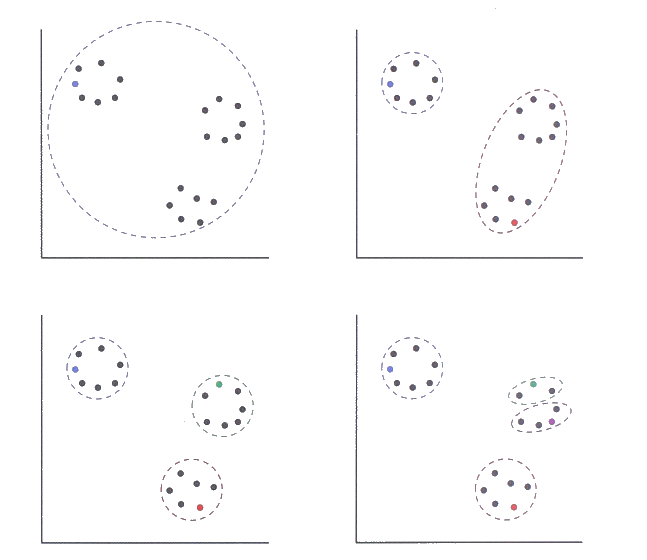
\includegraphics[width=8cm]{bio6.png}
    \caption{Primena algoritma \emph{Farthest Fast Traversal}}
    \label{slika 7}
\end{figure}
\\

Algoritam \textbf{FarthestFirstTraversal}:
\\
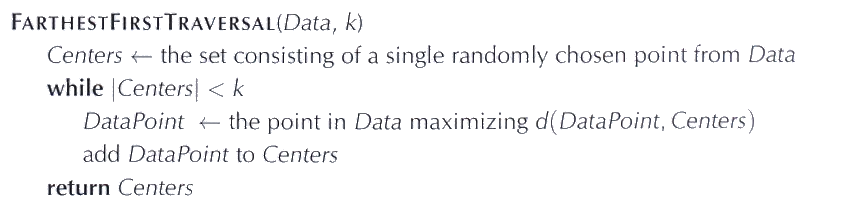
\includegraphics[width=\textwidth]{algoritam1.png}
\\

Algoritam \textbf{FarthestFirstTraversal} je brz i rešenje do kojeg dolazi najbolje aproksimira problem $k$-centar klasterovanja. Me\dj utim, ovaj algoritam se retko koristi u analizi genske ekspresije, jer biologe uglavnom zanimaju tipična, a ne maksimalna odstupanja. Da li možemo da predefinišemo naš problem tako više odgovara biolozima?


\subsection{$k$-means klasterovanje}

\subsubsection{Kvadrat distorzije greške}

Neka je dat skup $Data$ od $n$ tačaka podataka i skup $Centers$ od $k$ centara.  \textbf{Kvadrat distorzije greške} skupa $Data$ u odnosu na skup $Centers$ definišemo kao srednjekvadratno rastojanje od svake tačke podatka do njoj najbližeg centra. 

$$Distortion(Data, Centers) = \frac{1}{n} \sum_{\text{all points }DataPoint\text{ in }Data} d(DataPoint, Centers)^2$$

Možemo primetiti da u $MaxDistance$ učestvuje samo jedna tačka podatak, dok u $Distortion$ učestvuju sve tačke (Slika \ref{slika 8}).
\begin{figure}[h]
    \centering
    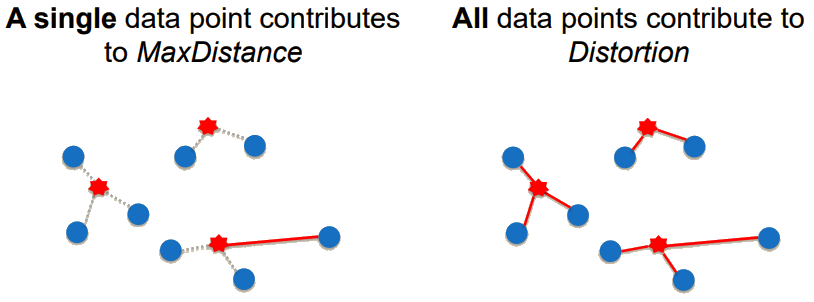
\includegraphics[width=8cm]{bio7.png}
    \caption{Razlika izme\dj u $MaxDistance$ i $Distortion$}
    \label{slika 8}
\end{figure}

Sada možemo definisati naš problem.

\begin{tcolorbox}
\textbf{Problem kvadrata distorzije greške:} Izračunati kvadrat distorzije greške skupa tačaka podataka u odnosu na skup centara.\\
\textit{Ulaz:} Skup tačaka $Data$ i skup centara $Centers$.\\
\textit{Izlaz:} Kvadrat distorzije greške $Distortion(Data, Centers)$.
\end{tcolorbox}

Ovo nas dovodi do modifikacije problema k-centar klasterovanja.

\begin{tcolorbox}
\textbf{Problem k-means klasterovanja:} Od datog skupa tačaka podatka, naći k centara tako da minimizuju kvadrat distorzije greške.\\
\textit{Ulaz:} Skup tačaka $Data$ i ceo broj $k$.\\
\textit{Izlaz:} Skup $k$ centara $Centers$ koji minimizuju $Distortion(Data, Centers)$.
\end{tcolorbox}

\subsubsection{k-means klasterovanje i centar gravitacije}

Ispostavlja se da je, za $k>1$, problem k-means klasterovanja NP-težak. Me\dj utim, kada je $k=1$, ovaj problem se svodi na pronalaženje jednog centra $x$ koji minimizuje kvadrat distorzije greške. 

Iako je podela skupa tačaka u jedan klaster trivijalan problem, i dalje nije sasvim jasno kako naći jedan centar koji minimizuje kvadrat distorzije greške. Rešavanje ovog, jednostavnijeg, problema će nam pomoći pri izradi heuristike kada je $k>1$.

\textbf{Centar gravitacije} skupa $Data$ je tačka čija $i$-ta koordinata predstavlja prosek $i$-tih koordinata svih tačaka iz $Data$.
$$\sum_{\text{all points }DataPoint\text{ in }Data}\frac{DataPoint}{|points in Data|}$$

Na slici \ref{slika 9} je crvenom bojom prikazan centar gravitacije tačaka $(2,3)$, $(4,1)$ i $(6,5)$.
$$ \bigg(\frac{2+4+6}{3}, \frac{3+1+5}{3}\bigg) = (4,3)$$
\begin{figure}[h]
    \centering
    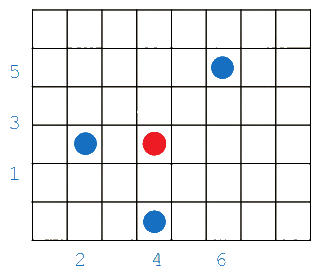
\includegraphics[width=7cm]{bio10.png}
    \caption{Centar gravitacije tačaka $(2,3)$, $(4,1)$ i $(6,5)$}
    \label{slika 9}
\end{figure}

\begin{teorema}[Teorema o centru gravitacije]{Centar gravitacije skupa tačaka $Data$ jeste jedina tačka koja je rešenje $1$-means problema klasterovanja.}
\end{teorema}

\section{Lojdov algoritam}

Na početku označimo proizvoljnih $k$ tačaka iz skupa $Data$ kao centre, a zatim ponavljamo sledeća dva koraka:

\begin{itemize}
\item \textbf{Od centara do klastera}: Nakon što su centri odre\dj eni, dodelimo svaku od tačaka podataka klasteru koji odgovara najbližem centru; veze su proizvoljno raskinute.

\item \textbf{Od klastera do centara}: Nakon što su tačke dodeljene klasterima, označimo centar gravitacije svakog klastera kao novi centar klastera.
\end{itemize}
 
Postupak se završava kada centri prestanu da se pomeraju. Možemo reći da tada Lojdov algoritam konvergira.
 
Prikažimo postupak na primeru, radi lakšeg razumevanja. Opisaćemo kako Lojdov algoritam radi za $k=3$ (slika \ref{slika 10}). 
U delu slike koji je označen sa 1 smo izabrali proizvoljne tri tačke kao centre (crvena, plava i zelena tačka). Zatim, dodeljujemo svaku tačku najbližem centru, praveći tako klastere (2). Nakon toga, prelazimo na korak \textbf{Od klastera do centara}, u kojem za nove centre klastera biramo centre gravitacije postojećih klastera. Pomeranje tih centara je prikazano na delu slike označenim sa 3. Sada, ponavljamo ova dva koraka. Na delu 4 primećujemo da su se klasteri promenili, a na delu 5 da su se plavi i zeleni centar pomerili, ali ne i crveni. Kada ponovo odredimo klastere (6), vidimo da su isti kao i u delu 4, dakle algoritam konvergira i postupak se završava.
%\newpage
\begin{figure}[h!]
    \centering
    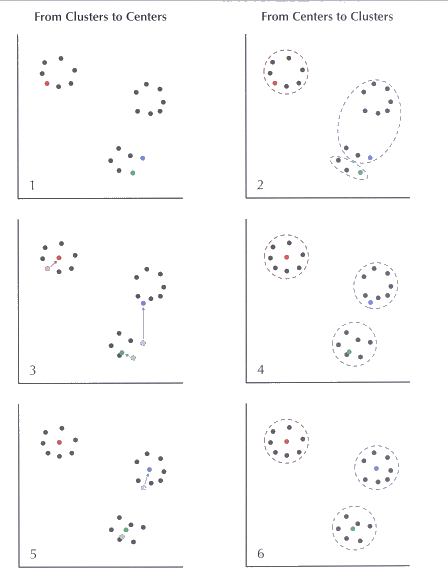
\includegraphics[width=10cm]{bio8.png}
    \caption{Lojdov algoritam u akciji za $k=3$}
    \label{slika 10}
\end{figure}

Da li Lojdov algoritam mora da konvergira?
\begin{figure}[h!]
    \centering
    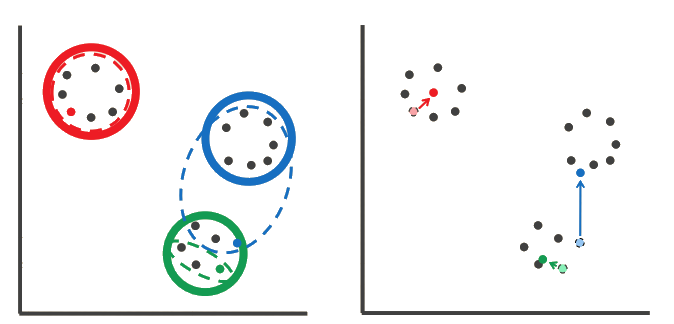
\includegraphics[width=10cm]{bio11.png}
    \caption{Prikaz smanjenja kvadrata distorzije greške u oba koraka Lojdovog algoritma}
    \label{slika 11}
\end{figure}


Ako je tačka podatak dodeljena novom centru u toku koraka \textbf{Od centara do klastera} kvadrat distorzije greške je smanjen jer ovaj centar mora biti bliži tački od prethodnog centra (slika \ref{slika 11} - prvi deo). Ako je centar pomeren u koraku \textbf{Od klastera do centara} kvadrat distorzije greške je opet smanjen jer je, prema teoremi o centru gravitacije, centar gravitacije jedina tačka koja minimizuje distorziju (slika \ref{slika 11} - drugi deo). Me\dj utim, može se desiti da se kvadrat distorzije greške smanjuje u svakom koraku sve manje i manje, što dovodi do beskonačnog procesa.


Napomenimo samo da, iako je rečeno da se na početku proizvoljno biraju centri, postoje bolji načini za inicijalizovanje. Naime, ukoliko napravimo loš izbor prvih centara, može se desiti da Lojdov algoritam veoma brzo konvergira, ali kao rezultat daje pogrešne klastere. Takav primer možemo videti na slici \ref{slika 12}.
\begin{figure}[h!]
    \centering
    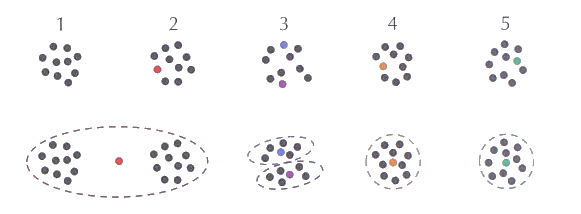
\includegraphics[width=10cm]{bio12.png}
    \caption{Primer lošeg inicijalizovanja centara}
    \label{slika 12}
\end{figure}


\subsection{Klasterovanje gena implicirano u diauxic smeni}

Kako izbor biološki relevantne vrednosti za $k$ može biti izazovno, mi ćemo, donekle proizvoljno, izabrati da podelimo 230 gena kvasca u šest klastera, što je prikazano na slici \ref{slika 13}. Primenjen je Lojdov algoritam na skup podataka koji sadrži 230 gena. Kao rezultat dobijeno je šest klastera koji prikazuju šest različitih tipova  ponašanja koji su uključeni u diauxic smenu i sadrže 37, 36, 58, 19, 36 i 44 gena, redom.
\begin{figure}[h!]
    \centering
    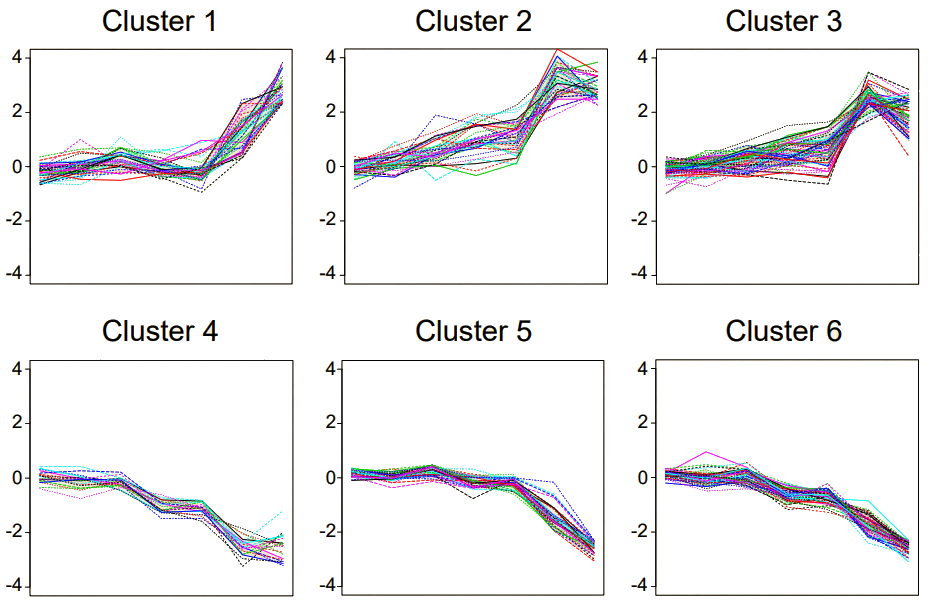
\includegraphics[width=10cm]{bio13.png}
    \caption{Podela gena kvasca na šest klastera}
    \label{slika 13}
\end{figure}

\section{Od tvrdog do mekog klasterovanja}
\subsection{Ograničenja k-means klasterovanja}

Sada kada smo se upoznali sa Lojdovim algoritmom, može nam se učiniti da je klasterovanje lako. Me\dj utim, pogledajmo prvi deo slike \ref{slika 14} i razmislimo kako bismo klasterovali date tačke. U središnjem delu vidimo kako bi ljudsko oko klasterovalo, a u poslednjem redu kako to čini Lojdov algoritam. Primećujemo da dolazi do neslaganja, što je čest slučaj.
\begin{figure}[h!]
    \centering
    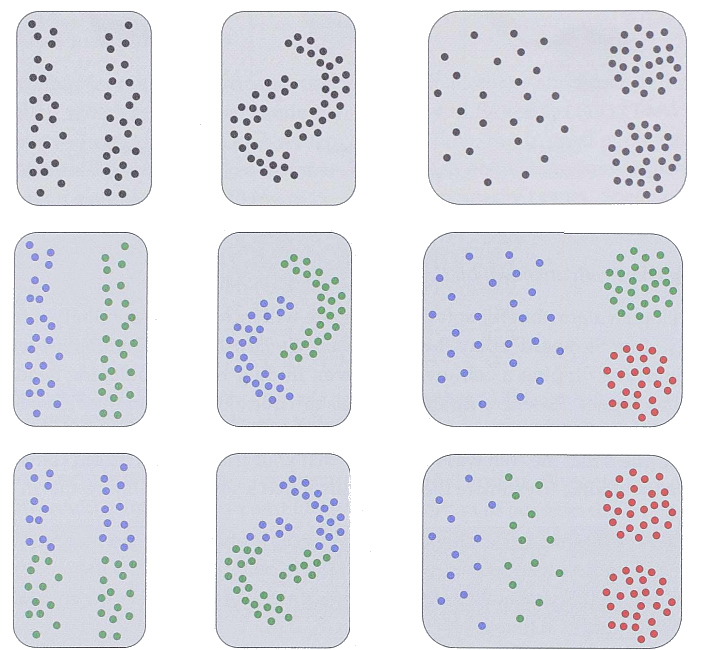
\includegraphics[width=10cm]{bio14.png}
    \caption{Razlika u klasterovanju ljudskim okom i Lojdovim algoritmom}
    \label{slika 14}
\end{figure}

Slabost formulacije problema k-means klasterovanja je u tome što neku tačku dodeljuje samo jednom klasteru, tj. vrši se tzv. \textbf{tvrdo klasterovanje} (slika \ref{slika 15} gore).  \textbf{Središnja tačka} jeste tačka koja se nalazi približno na pola puta izme\dj u dva klastera. Da li možemo središnju tačku da dodelimo dvama klasterima? Da li se može izvršiti tzv. \textbf{meko klasterovanje} (slika \ref{slika 15} dole)? 
\begin{figure}[h!]
    \centering
    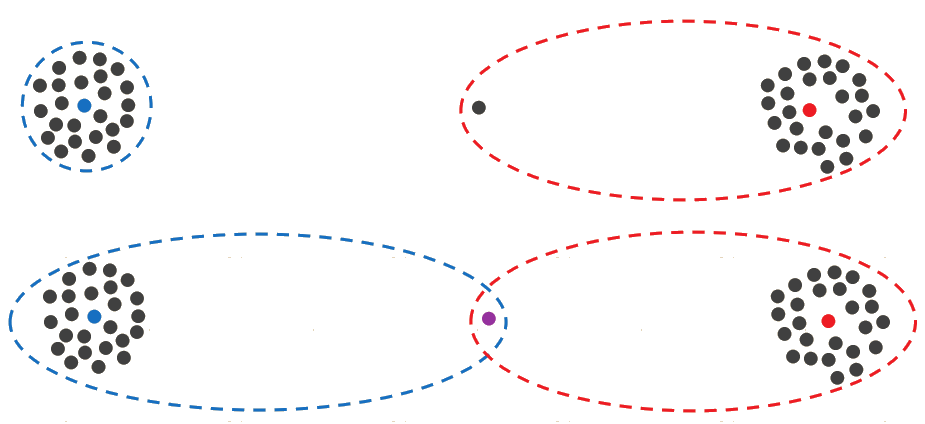
\includegraphics[width=8cm]{bio15.png}
    \caption{Tvrdo i meko klasterovanje; središnja tačka je označena ljubičastom bojom}
    \label{slika 15}
\end{figure}

Na levom delu slike \ref{slika 16}, imamo tačke podeljene u dva klastera pomoću Lojdovog algoritma. Tačke su prikazane plavom ili crvenom bojom, u zavisnosti od toga kom klasteru pripadaju. Meko klasterovanje je prikazano na desnom delu iste slike. Svakoj tački je dodeljen ure\dj eni par $(r_{blue}, r_{red})$ koji predstavlja procenat plave i crvene boje u datoj tački koji se dobija na osnovu vrednosti $"responsibility"$ svakog klastera za datu tačku. Mora da važi $r_{blue} + r_{red} = 1$.
\begin{figure}[h!]
    \centering
    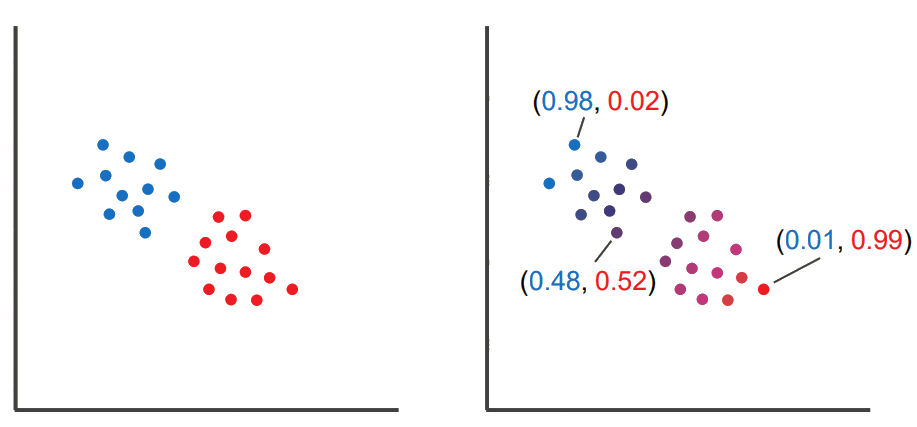
\includegraphics[width=8cm]{bio16.png}
    \caption{Tvrdo i meko klasterovanje}
    \label{slika 16}
\end{figure}

\section{Od bacanja novčića do k-means klasterovanja}
\subsection{Bacanje novčića sa nepoznatim otežanjem}
Da bismo došli do algoritma za meko klasterovanje, moramo se upoznati sa naizgled nepovezanom analogijom.

Pretpostavimo da bacamo otežani novčić, sa nepoznatim otežanjem $\theta$ i da od $n$ bacanja glava padne $i$ puta. Za svako otežanje $\theta$ izme\dj u 0 i 1, možemo izračunati verovatnoću dobijene sekvence bacanja. Potrebno je da na\dj emo $\theta$ koje maksimizuje ovu verovatnoću.

Čini se da je najbolje da za $\theta$ izaberemo broj pojavljivanja glave podeljen sa ukupnim brojem bacanja, odnosno, $\theta = \frac{i}{n}$. Kako smo došli do ovoga?

Verovatnoća generisanja date sekvence bacanja je 
$$Pr(sequence|{\theta}) = {\theta}^i \cdot (1-{\theta})^{n-i}.$$
Označimo je sa $f(\theta)$. Kako tražimo $\theta$ koje maksimizuje datu verovatnoću, izjednačićemo izvod funkcije $f$ sa 0.
\begin{equation}
\begin{split}
f’(\theta) & = (\theta^i \cdot (1-\theta)^{n-i})'\\
	  & = (\theta^i)’ \cdot (1-\theta)^{n-i} + \theta^i \cdot ((1-\theta)^{n-i})'\\
	  & = i \cdot \theta^{i-1} \cdot (1-\theta)^{n-i} - (n-i)\theta^i \cdot (1-\theta)^{n-i-1}\\
	  & = \theta^{i-1} \cdot (i(1-\theta)^{n-i} - (n-i)\theta(1-\theta)^{n-i-1})\\
	  & = \theta^{i-1} \cdot (1-\theta)^{n-i-1} \cdot (i(1-\theta)-(n-i)\theta)\\
	  & = \theta^{i-1} \cdot (1-\theta)^{n-i-1} \cdot (i-i\theta-n\theta+i\theta)\\
	  & = \theta^{i-1} \cdot (1-\theta)^{n-i-1} \cdot (i-n\theta)\\
\end{split}
\end{equation}
$f’(\theta)=0, za \hspace{0.2cm} \theta=0, \theta=1, \theta=\frac{i}{n}$ 

Kako bi problem bacanja novčića bio interesantniji, bacaćemo dva novčića $A$ i $B$ koja izgledaju identično ali imaju različita otežanja $\theta_A$ i $\theta_B$, birajući slučajno novčić koji se baca. Nakon posmatranja serije bacanja, naš zadatak je da procenimo $\theta_A$ i $\theta_B$, koje nazivamo \textbf{parametrima}. Problem pojednostavljujemo tako što ćemo pretpostaviti da nakon svakih $n$ bacanja zadržavamo postojeći novčić ili uzimamo drugi. Pet serija od po $n = 10$ bacanja su prikazana na slici \ref{slika 17}; verovatnoće da je pala glava prikazujemo sledećim vektorom:
$$
Data = (0.4, 0.9, 0.8, 0.3, 0.7)
$$
\begin{figure}[h!]
    \centering
    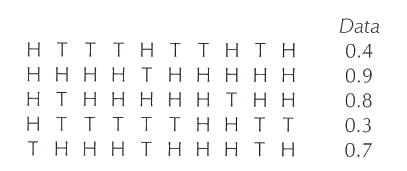
\includegraphics[width=8cm]{bio17.png}
    \caption{Primer 5 serija sa po 10 bacanja novčića}
    \label{slika 17}
\end{figure}

Ako znamo da je novčić $A$ korišćen u prvoj i u četvrtoj seriji, dobijamo da je $\theta_A=(0.4+0.3)/2=0,35$, a da je $\theta_B=(0.9+0.8+0.7)/3=0.8$. Predstavljamo izbor novčića kao binarni vektor $HiddenVector=(1,0,0,1,0)$, gde $1$ na $k$-toj poziciji označava da je novčić $A$ korišćen u $k$-toj sekvenci bacanja, a $0$ da je korišćen novčić $B$. Ova notacija nam omogućava da napišemo jednačine za parametre u zavisnoti od vektora $Data$ i $HiddenVektor$ ($\overrightarrow{1}$ se odonosi na jedinični vektor odre\dj ene dužine):

\begin{equation}
\label{eq2}
\begin{split}
\theta_A = \frac{\sum_i HiddenVector_i \cdot Data_i}{\sum_i HiddenVector_i} & = 
\frac{HiddenVector \cdot Data}{\overrightarrow{1} \cdot HiddenVector} \\
\theta_B = \frac{\sum_i (1-HiddenVector_i) \cdot Data_i}{\sum_i (1-HiddenVector_i)} & =
\frac{(\overrightarrow{1} - HiddenVector) \cdot Data}{\overrightarrow{1} \cdot (\overrightarrow{1} - HiddenVector)}
\end{split}
\end{equation}

Ako su nam dati vektori $Data$ i $HiddenVector$ možemo dobiti parametre, a ako su nam dati paramtri i vektor $Data$ da li možemo odrediti $HiddenVector$? Ako nam je data vrednost parametara, odre\dj ivanje vrednosti za $HiddenVector$ odgovara odre\dj ivanju da li bacanje novčića $A$ ili novčića $B$ ima veću verovatnoću da generiše $n$ prikazanih bacanja u svakoj od 5 serija. Ako pretpostavimo da su vrednosti parametara $(\theta_A,\theta_B) = (0.6,0.82)$ za petu seriju bacanja dobijamo da je verovatnoća korišćenja novčića $A$ približno jednaka $\theta_A^7\cdot(1-\theta_A^3) \approx 0.00179$, a da je verovatnoća korišćenja novčića $B$ približno jednaka $\theta_B^7\cdot(1-\theta_B^3) \approx 0.00145$. Kako je $0.00179 > 0.00145$ postavaljamo petu vrednost vektora $HiddenVector$ na $1$. Označimo sa $Pr(Data_i\mid \theta)$ uslovnu verovatnoću generisanja ishoda $Data_i$ bacanjem novčića sa težinom $\theta$.
$$
Pr(Data_i\mid \theta) = \theta^{n \cdot Data_i}\cdot(1-\theta)^{n \cdot (1-Data_i)}
$$
Ako je $Pr(Data_i\mid \theta_A) > Pr(Data_i\mid \theta_B)$ onda je novčićem $A$ verovatno generisana $i$-ta serija bacanja, i na osnovu toga postavljamo vrednost $HiddenVector_i$ na $1$. U suprotnom postavljamo vrednost $HiddenVector_i$ na $0$.

Ako nam je poznata vrednost vektora $HiddenVector$, a nije nam poznata vrednost parametara, tada možemo rekonstruisati najverovatniju vrednost parametara. Ako nam je data  vrednost parametara, mi možemo rekonstruisati najverovatniju vrednost vektora $HiddenVector$. Naš originalni problem je bio da su i vrednosti parametara $(\theta_A,\theta_B)$ i vrednosti vektora $HiddenVector$ nepoznate. 

Pronalaženje vrednosti parametara i vektora $HiddenVector$ se može činiti beznadežno, ali smo naučili da polaženje od nasumične vrednosti ne mora nužno da bude loša ideja. Krenućemo od nasumičnih vrednosti parametara i rekonstruisati $HiddenVector$. Nakon dobijene vrednosti za $HiddenVector$ izračunaćemo vrednosti parametara, itd. Na koji problem nas ovo podseća (slika \ref{slika 18})? 
\begin{figure}[h!]
    \centering
    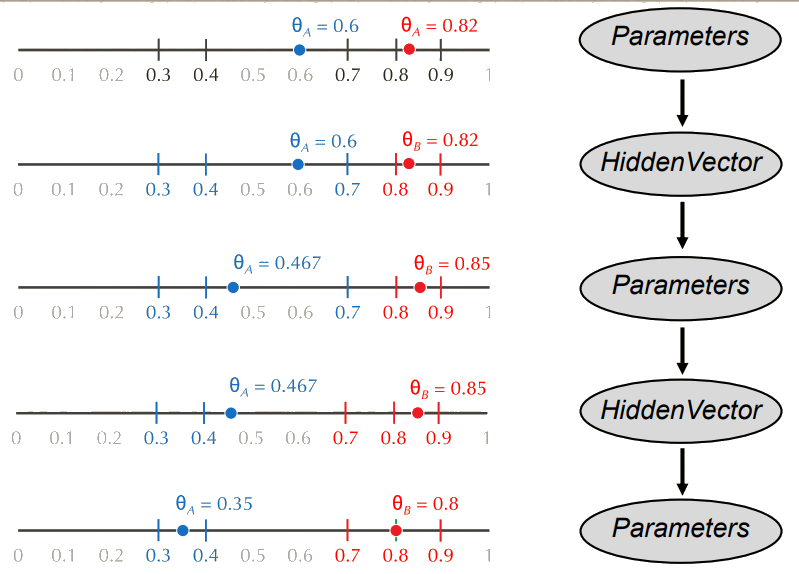
\includegraphics[width=10cm]{bio18.png}
    \caption{Primer primene algoritma$ $ $"$bacanja novčića$"$ $ $ sa početnom vrednosti parametara $(0.6, 0.82)$}
    \label{slika 18}
\end{figure}

Neka je dato $n$ tačaka u $m$-dimenzionom prostoru $Data = (Data_1,\dots, Data_n)$, predstavljamo njihovo klasterovanje u $k$ klastera kao $n$-dimenzioni vektor $HiddenVector = (HiddenVector_1,\dots, \\ HiddenVector_n ),$ gde svaki $HiddenVector_i$ uzima vrednosti od $1$ do $k$. Nakon toga predstavljamo $k$ centara kao $k$ tačaka u $m$-dimenzionom prostoru, parametri $(\theta_1,\dots,\theta_k)$. Kod Lojdovog algoritma krećemo od nasumično izabranih vrednosti parametara i onda nastavljamo sa sledeća dva koraka:
\begin{itemize}
    \item \textbf{Od centara do klastera}: parametri $\rightarrow HiddenVector$
    \item \textbf{Od klastera do centara}: $HiddenVector \rightarrow $ parametri 
\end{itemize}

Jedina razlika izme\dj u Lojdovog algoritma za k-means klasterovanje i algoritma bacanja novčića je u tome kako se izvršava korak \textbf{Od centara do klastera}. U prvom dodeljujemo tačku klasteru na osnovu najbližeg centra, a u drugom računamo $HiddenVector_i$ upore\dj ujući $Pr(Data_i|\theta_A)$ sa $Pr(Data_i|\theta_B)$.

\section{Meko odlučivanje u bacanju novčića} % Meko?
\subsection{Očekivanje maksimizacije: E-korak}

Iskoristićemo opisanu analogiju sa bacanjem novčića da do\dj emo do meke verzije k-means klasterovanja. Neka je dato $Parameters = (\theta_A, \theta_B)$. Možemo doneti tzv. teške odluke za $HiddenVector$ upore\dj ujući $Pr(Data_i|\theta_A)$ sa $Pr(Data_i|\theta_B)$. Me\dj utim, na osnovu ovoga ne možemo znati koji novčić je korišćen. Ako su $Pr(Data_i|\theta_B)$ i $Pr(Data_i|\theta_A)$ približno jednaki, onda će pouzdanost da je korišćen novčić $B$ biti približno $50$. S druge strane, ako je $Pr(Data_i|\theta_B)$ mnogo veće od $Pr(Data_i|\theta_A)$, onda možemo biti skoro sigurni da je korišćen novčić $B$.
Dakle, možemo govoriti o pouzdanosti da je neki novčić korišćen kao o "odgovornosti" tog novčića za datu sekvencu bacanja. 

Pokazaćemo na primeru kako računamo odgovornosti novčića. Neka je dato $Parameters = (\theta_A, \theta_B) = (0.6, 0.82)$ i sekvenca bacanja "THHHTHHHTH", gde H predstavlja glavu, a T pismo. Prvo ćemo izračunati $Pr(0.7|\theta_A)$ i $Pr(0.7|\theta_B)$
    
$$Pr(0.7|\theta_A) = 0.6^7 \cdot 0.4^3 \approx 0.00179$$ 
$$Pr(0.7|\theta_B)= 0.82^7 \cdot 0.18^3 \approx 0.00145$$

Ranije bismo strogo zaključili da je verovatno korišćen novčić $A$, ali sada, kako je verovatnije da novčić $A$ generiše sedam glava iz deset bacanja, dodeljujemo veću odgovornost novčiću $A$. % Ovo mnogo glupo zvuči
Jedan od načina kako dodeljujemo odgovornosti prikazan je narednim formulama:
$$\frac{Pr(0.7|\theta_A)}{Pr(0.7|\theta_A) + Pr(0.7|\theta_B)} = \frac{0.00179}{0.00179 + 0.00145} \approx 0.55 $$
$$\frac{Pr(0.7|\theta_B)}{Pr(0.7|\theta_A) + Pr(0.7|\theta_B)} = \frac{0.00145}{0.00179 + 0.00145} \approx 0.45 $$

Umesto $HiddenVector$-a, kao rezultat imamo matricu odgovornosti, $HiddenMatrix$, dimenzije $2 \times 5$, %responsibility profile
koja se može konstruisati na osnovu $Data$ i $Parametres$
$$(Data, ? ,Parametres) \rightarrow HiddenMatrix.$$

Ova promena predstavlja tzv. \textbf{E-korak}. Na slici \ref{slika 19}, prikazano je kako od $Data = (0.4, 0.9, 0.8, 0.3, 0.7)$ i $Parametres = (0.6, 0.82)$ dobijamo $HiddenMatrix$. U nastavku će biti reči o \textbf{M-koraku}, u kome od $HiddenMatrix$ i $Data$, dobijamo izmenjene parametre $Parametres'$.
%slika 8,20
\begin{figure}
    \centering
    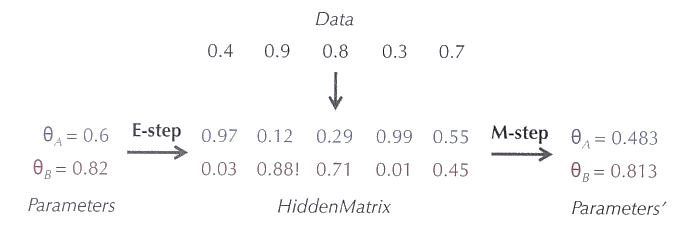
\includegraphics[width=10cm]{bio19.png}
    \caption{E-korak i M-korak}
    \label{slika 19}
\end{figure}

\subsection{Očekivanje maksimizacije: M-korak}

Do sada smo parametre $Parameters$ računali pomoću formula (\ref{eq2}). Kod mekog dodeljivanja, primetimo da generisanje ishoda kod dva novčića može biti predstavljeno binarnom matricom odgovornosti.
$$HiddenMatrix \hspace{0.2cm}
\begin{matrix}
0 & 1 & 1 & 0 & 1 \\
1 & 0 & 0 & 1 & 0
\end{matrix}
$$
$1$ u $i$-toj koloni u prvom redu označava da je novčić $A$ generisao ishod u $i$-tom bacanju, a $1$ u $i$-toj koloni u drugom redu, da je $i$-ti ishod generisao novčić $B$.
Možemo primetiti da je prvi red, koji označavamo sa $HiddenMatrix_A$ ustvari $HiddenVector$, a da drugi red, $HiddenMatrix_B$ ustvari predstavlja $\overrightarrow{1} - HiddenVector$. Zato možemo izmeniti dosadašnje formule (\ref{eq2}) sa:
\begin{equation}
\label{eq3}
\begin{split}
\theta_A = \frac{HiddenMatrix_A \cdot Data}{\overrightarrow{1} \cdot HiddenMatrix_A}\\
\theta_B =\frac{HiddenMatrix_B \cdot Data}{\overrightarrow{1} \cdot HiddenMatrix_B}
\end{split}
\end{equation}
	
Izračunajmo izmenjene vrednosti za $Parameters$ sa slike \ref{slika 19}, prema novim formulama. 
$$\theta_A = \frac{0.97 \cdot 0.4 + 0.12 \cdot 0.9 + 0.29 \cdot 0.8 + 0.99 \cdot 0.3 + 0.55 \cdot 0.7}{0.97 + 0.12 + 0.29 + 0.99 + 0.55} = \frac{1.41}{2.92} \approx 0.483$$

$$\theta_B = \frac{0.03 \cdot 0.4 + 0.88 \cdot 0.9 + 0.71 \cdot 0.8 + 0.01 \cdot 0.3 + 0.45 \cdot 0.7}{0.03 + 0.88 + 0.71 + 0.01 + 0.45} = \frac{1.69}{2.08} \approx 0.813$$

Ova promena, $(Data, HiddenMatrix, ?) \rightarrow Parameters$, 	predstavlja tzv. \textbf{M-korak}.

\subsection{Algoritam očekivanja maksimizacije}

Nakon što smo se upoznali sa E-korakom i M-korakom, možemo konstruisati algoritam očekivanja maksimizacije.
Na početku se proizvoljno biraju parametri $Parameters$. Zatim se naizmenično izvršavaju E-korak, u kojem računamo matricu odgovornosti $HiddenMatrix$ na osnovu $Data$ i $Parameters$:
$$(Data, ?, Parameters) \rightarrow HiddenMatrix$$
i M-korak, u kojem ponovo procenjujemo $Parameters$ koristeći $HiddenMatrix$:
$$(Data, HiddenMatrix, ?) \rightarrow Parameters$$
 	
\section{Meko k-means klasterovanje}

Uveli smo očekivanje maksimizacije kako bismo izmenili Lojdov algoritam i tako dobili \textbf{algoritam za meko k-means klasterovanje}. Na početku proizvoljno izaberemo centre, a zatim iterativno izvršavamo sledeća dva koraka, koja će u nastavku biti detaljnije opisana:

\begin{itemize}
    \item \textbf{Od centara do mekih klastera (E-korak)}: Nakon što smo izabrali centre, dodeljujemo svakoj tački podatku "odgovornost" \ za svaki klaster, gde veća odgovornost odgovara jačoj pripadnosti klasteru.
    \item \textbf{Od mekih klastera do centara (M-korak)}: Nakon što su tačke dodeljene klasterima, računamo nove centre.
\end{itemize}

Krećemo od koraka \textbf{Od centara do mekih klastera}. Što je tačka bliža centru, to centar jače "privlači" \ tu tačku, kao što zvezda jače privlači planetu ukoliko joj je ona bliža. Neka je dato $k$ centara $Centers = (x_1, \dots, x_k)$ i $n$ tačaka $Data = (Data_1, \dots, Data_n)$. Potrebno je, od ovih podataka, konstruisati matricu odgovornosti $HiddenMatrix$, gde $HiddenMatrix_{i,j}$ označava privlačnost centra $i$ na tačku $j$. %je l se ovako kaye
Ovu privlačnost možemo izračunati pomoću Njutnovog zakona gravitacije sa inverznim kvadratima,
$$HiddenMatrix_{i,j} = \frac{1/d(Data_j, x_i)^2}{\sum_{all centers x_i} 1/d(Data_j, x_i)^2}.$$
Me\dj utim, u praksi se pokazalo bolje računanje preko \textbf{funkcije particije} iz statičke fizike:
$$HiddenMatrix_{i,j} = \frac{e^{-\beta \cdot d(Data_j, x_i)}}{\sum_{all centers x_i} e^{-\beta \cdot d(Data_j, x_i)}},$$
gde je $\beta$ parametar koji odražava količinu fleksibilnosti u mekom dodeljivanju i koji nazivamo \textbf{parametrom krutosti (stiffness parameter)}. Na slici \ref{slika 20} je prikazan primer dobijanja različitih vrednosti u matrici $HiddenMatrix$ za različito $\beta$ prema podacima $Data = (-3,-2,-1,0,1,2,3)$ i centrima $Centers = (-2.5,2.5)$.
	

\begin{figure}
    \centering
    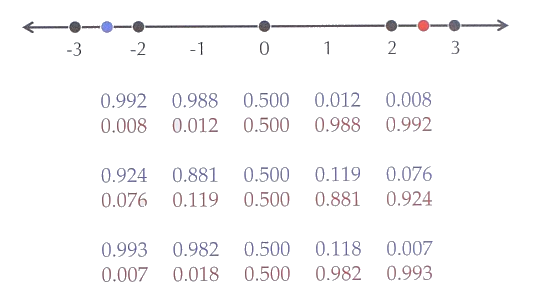
\includegraphics[width=10cm]{bio20.png}
    \caption{Tri verzije konstrukcije $HiddenMatrix$ matrice: 1) korišćenjem Njutnovog zakona inverznim kvadratima; 2) preko funkcije particije sa parametrom krutosti $\beta = 0.5$; 3) preko funkcije particije sa parametrom krutosti $\beta = 1$}
    \label{slika 20}
\end{figure}

Sada ćemo opisati korak \textbf{Od mekih klastera do centara}. Podsetimo se formula (\ref{eq3}) iz M-koraka za $\theta_A$ i $\theta_B$.
U mekom k-means klasterovanju, ako sa $HiddenMatrix_i$ označimo $i$-ti red matrice $HiddenMatrix$, možemo ažurirati centar $x_i$ koristeći analogiju sa navedenim formulama.
Specijalno, $j$-ta koordinata centra $x_i$, u oznaci $x_{i,j}$ može se izračunati kao:
$$x_{i,j} = \frac{HiddenMatrix_i \cdot Data^j}{HiddenMatrix_i \cdot \overrightarrow{1}},$$
gde $Data^j$ predstavlja $n$-dimenzioni vektor koji za elemente ima $j$-te koordinate svih $n$ tačaka iz $Data$. Izmenjeni centar $x_i$	nazivamo \textbf{težinskim centrom gravitacije} tačaka $Data$.

Na osnovu podataka sa slike \ref{slika 20}, možemo izračunati otežane centre gravitacije za matricu $HiddenMatrix$ i tako dobijamo nove, ažurirane, centre.
$$x_1 = \frac{0.993 \cdot (-3) + 0.982 \cdot (-2) + 0.500 \cdot (0) + 0.018 \cdot (2) + 0.007 \cdot (3)}{0.993 + 0.982 + 0.500 + 0.018 + 0.007} = -1.955$$
$$x_2 = \frac{0.007 \cdot (-3) + 0.018 \cdot (-2) + 0.500 \cdot (0) + 0.982 \cdot (2) + 0.993 \cdot (3)}{0.007 + 0.018 + 0.500 + 0.982 + 0.993} = 1.955$$	
	
Sada, kada smo upoznati sa svim ovim stvarima, možemo konstruisati algoritam očekivanja maksimizacije za meko k-means klasterovanje.

\section{Hijerarhijsko klasterovanje}

Prisetimo se da smo u Poglavlju 7 govorili o matrici rastojanja $D$. Sada ćemo videti kako istu matricu možemo koristiti pri podeli gena u klastere. Do sada smo pretpostavili da imamo fiksan broj klastera, $k$. Me\dj utim, u praksi veoma često klasteri imaju podklastere, koji imaju potpodklastere itd (slika \ref{slika 21}). Algoritam hijerarhijskog klasterovanja koristi matricu rastojanja $D$ veličine $n \times n$ kako bi organizovao $n$ tačaka u drvo. 
% slike sa slajdova 112,113,114	da se napravi jedna7
\begin{figure}
    \centering
    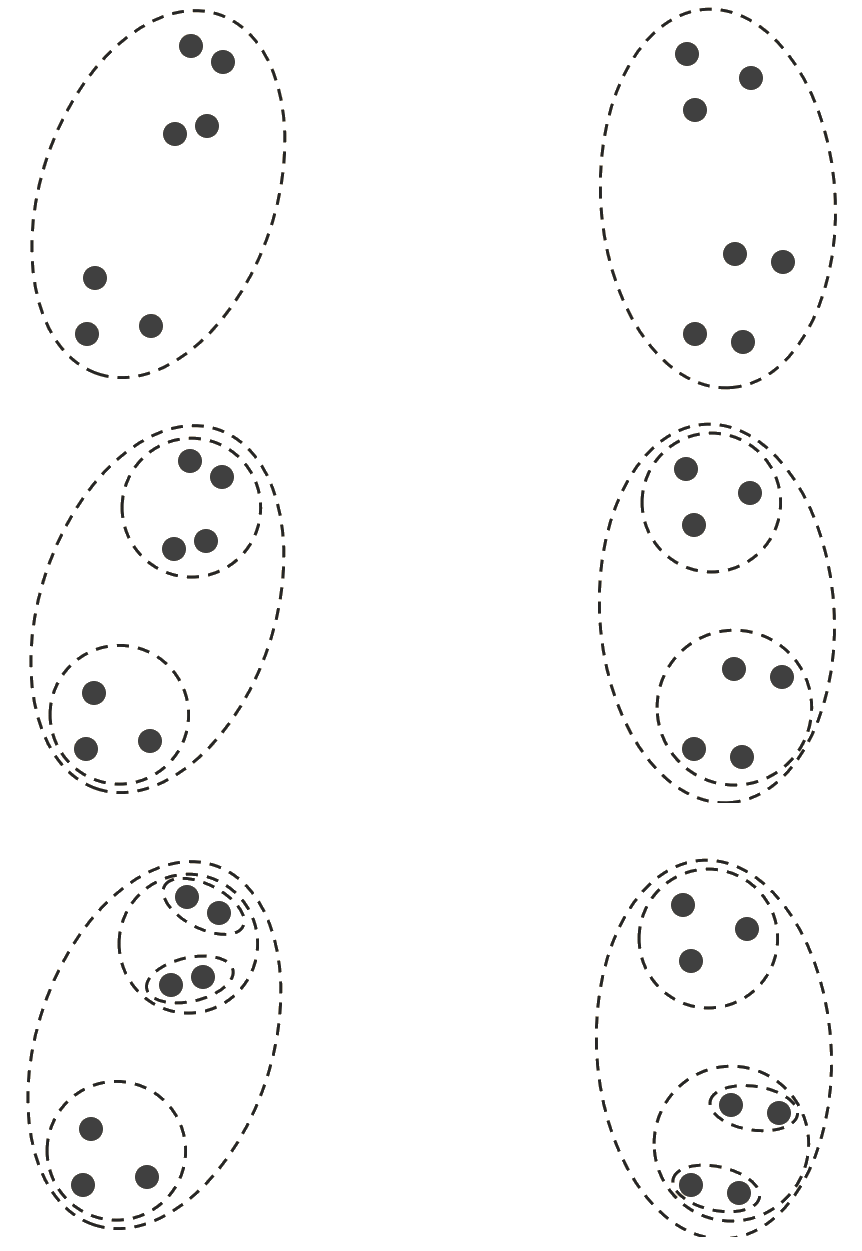
\includegraphics[width=10cm]{bio21.png}
    \caption{Klasteri, podklasteri i potpodklasteri}
    \label{slika 21}
\end{figure}

Algoritam hijerarhijskog klasterovanja počinje od transformacije ekspresione matrice veličine $n \times m$ u matricu rastojanja $D$ veličine $n \times n$. Ovaj algoritam postepeno transformiše $n$ različitih particija podataka u klastere, koji su predstavljeni drvetom u kome je svaki čvor označen klasterom. Prva particija ima $n$ jednočlanih klastera koji predstavljaju listove drveta, svaki element formira svoj klaster. Druga particija spaja dva najbliža klastera u zajednički dvočlani klaster. Uopšteno $i$-ta particija spaja dva najbiža klastera iz $(i-1)$-ve particije i ima $n-i+1$ klastera. Ovaj algoritam liči na UPGMA algritam (poglavlje 7).

Još uvek nismo definisali kako ovaj algoritam računa rastojanje $D(C_{new}, C)$ izme\dj u novog klastera $C_{new}$ i svakog starog klastera $C$. U praksi, algoritmi klasterovanja računaju ovo rastojanje na različite načine, i na osnovu toga daju različite rezultate. Jedan uobičajen pristup definiše rastojanje izme\dj u dva klastera kao najmanje rastojanje izme\dj u bilo kog para elemenata iz tih klastera. UPGMA algoritam koristi prosečno rastojanje izme\dj u elemenata u klasterima.
$$
D_{min}(C_1, C_2) = \min_{\text{all points } i \text{ in cluster }C_1\text{, all points } j \text{ in cluster }C_2}D_{i,j} 
$$
\\
Algoritam \textbf{Hijerarhijskog klasterovanja}:
\\
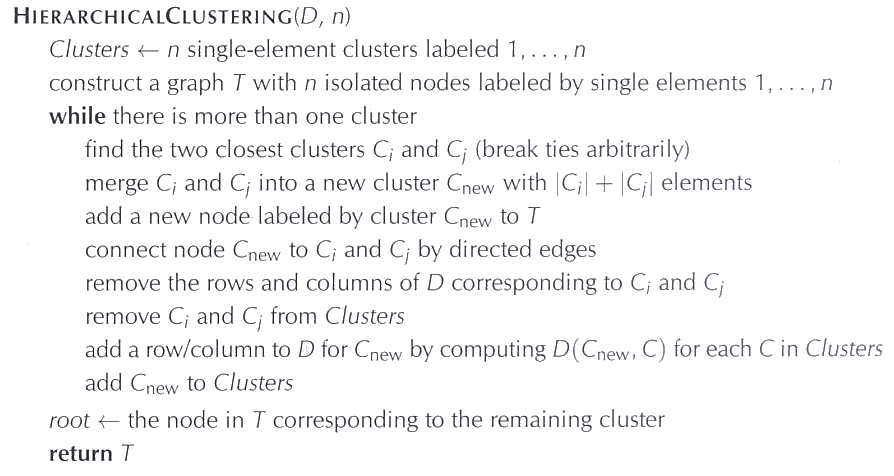
\includegraphics[width=\textwidth]{algoritam2.png}
\\

Objasnićemo rad algoritma na primeru (slika \ref{slika 22}). U gornjem levom uglu slike data je matrica rastojanja D i njen najmanji element je označen crvenom bojom. Vidimo da taj element odgovara genima $g_3$ i $g_5$. Dakle, spajamo ova dva klastera sa po jednim elementom u novi klaster $\{g_3,g_5\}$, što možemo primetiti u gornjem desnom uglu. U srednjem delu levo imamo izmenjenu matricu rastojanja, u kojoj smo izračunali $D_{min}$ za novi klaster. Opet je minimalna vrednost označena crveno. Nastavljamo postupak i sada spajamo klastere sa po jednim elementom $g_2$ i $g_4$ (središnji deo desno). U donjem delu slike, možemo videti kako algoritam nastavlja sa radom. Ponavljajući ovaj postupak, konstruiše se drvo koje odgovara matrici $D$.
\newpage
\begin{figure}[h!]
    \centering
    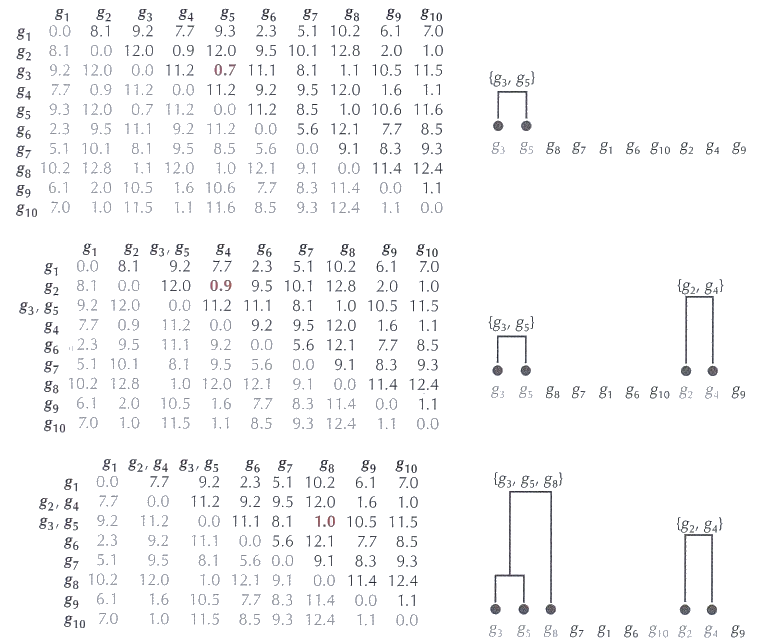
\includegraphics[width=\textwidth]{bio22.png}
    \caption{Primer rada algoritma hijerarhijskog klasterovanja}
    \label{slika 22}
\end{figure}
	
\section{Zadaci sa vežbi}
\setexamplecodestyle

U nastavku će biti predstavljeni zadaci sa vežbi na kursu rađeni u programskom jeziku Python.

\subsection{Farthest Fast Traversal}
\lstinputlisting[language=Python]{FarthestFirst.py}
\subsection{Hijerarhijsko klasterovanje}	
\lstinputlisting[language=Python]{HierarchicalCustering.py}
	
	
\end{document}

